% \section{实验过程}

% 本实验首先在香山仿真环境中基于 AM 编译示例程序，生成可在 NEMU 上运行的 RISC-V 裸机程序镜像；随后使用 NEMU 模拟器运行该程序，并通过开启内存访问日志功能获得程序执行过程中的内存地址访问序列，即 trace.log 文件。

% 在获得 trace.log 后，实验进一步编写 Cache 模拟器，以 trace.log 中记录的访存地址作为输入，按照给定的 Cache 容量、块大小、相联度和替换算法模拟 Cache 的访问过程，并统计总访问次数、命中次数、缺失次数以及命中率。

% 最后，通过改变 Cache 大小、Cache 块大小、相联度、替换算法、矩阵规模以及代码实现方式，观察不同配置下 Cache 命中率和 Miss 数的变化；在选做部分进一步使用香山性能计数器统计真实处理器微结构下的 Cache 行为，并与自行编写的 Cache 模拟器结果进行对比分析。

% 本实验的总体流程如下：

% \begin{enumerate}
%     \item 在 AM 环境中编译矩阵乘法程序，生成 RISC-V 可执行镜像；
%     \item 使用 NEMU 运行程序，并记录内存访问序列 trace.log；
%     \item 编写 Cache 模拟器，读取 trace.log 并模拟 Cache 命中与缺失过程；
%     \item 调整 Cache 参数和程序实现方式，统计不同配置下的 hit/miss 情况；
%     \item 根据实验数据分析 Cache 参数、替换算法和程序访存模式对命中率的影响。
%     \item 使用香山性能计数器统计 DCache 访存行为，并与软件 Cache 模拟器结果进行对比。
% \end{enumerate}

\subsection{Cache大小对命中率的影响}
\subsubsection{实验结果}
选取矩阵规模为128时的trace数据分析,固定映射方法为4路组相联、替换算法为"LRU",分别测试分组大小为$16B,64B,128B$在
Cache大小分别为$1,2,4,8,16,32,64,128KB$时的命中率,结果如下: % 数据来自data/capacity.csv
\begin{table}[htbp]
  \centering
  \caption{Cache大小对命中率的影响}
  \label{tab:cache_stats}
  \begin{tabular}{cccc} % 四列居中对齐
    \toprule
    Cache大小(KB) & 块大小(B) & 命中率 (\%) & Miss数 \\
    \midrule
    1   & 16  & 48.934697591460555 & 2171337 \\
    2   & 16  & 49.42544576429553  & 2150470 \\
    4   & 16  & 49.43146634857913  & 2150214 \\
    8   & 16  & 49.43974465196907  & 2149862 \\
    16  & 16  & 49.457806404819856 & 2149094 \\
    32  & 16  & 49.493929910521416 & 2147558 \\
    64  & 16  & 96.83107957307472  & 134745  \\
    128 & 16  & 99.42044820898201  & 24643   \\
    1   & 64  & 49.29104092374577  & 2156185 \\
    2   & 64  & 49.74862884720627  & 2136728 \\
    4   & 64  & 49.75163913934807  & 2136600 \\
    8   & 64  & 49.75239171238352  & 2136568 \\
    16  & 64  & 49.75765972363166  & 2136344 \\
    32  & 64  & 49.76650245679819  & 2135968 \\
    64  & 64  & 97.26987668855635  & 116087  \\
    128 & 64  & 99.85480043997302  & 6174    \\
    1   & 128 & 49.2675700522027   & 2157183 \\
    2   & 128 & 49.76130499927212  & 2136189 \\
    4   & 128 & 49.76431529141392  & 2136061 \\
    8   & 128 & 49.76431529141392  & 2136061 \\
    16  & 128 & 49.76431529141392  & 2136061 \\
    32  & 128 & 49.77033587569751  & 2135805 \\
    64  & 128 & 97.14652526446474  & 121332  \\
    128 & 128 & 99.92725911254236  & 3093    \\
    \bottomrule
  \end{tabular}
\end{table}
对应折线图如图:
\begin{figure}[H]
    \centering
    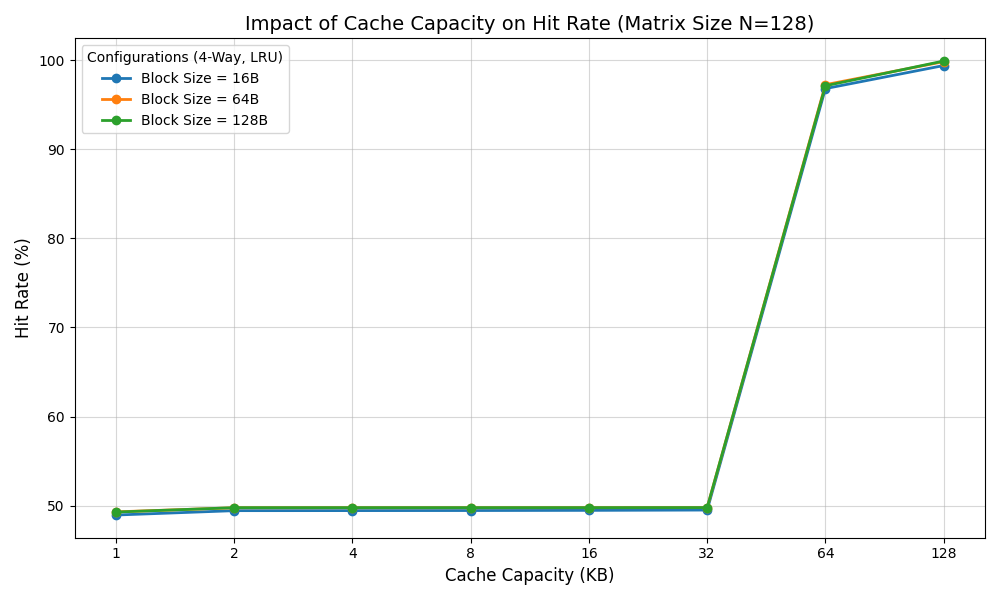
\includegraphics[width = 1\textwidth]{figure/capacity_impact_analysis.png}
    \caption{Cache大小对命中率的影响}
\end{figure}
\subsubsection{实验现象描述与分析}
\begin{itemize}
    \item 数据基础:在$N = 128$的int型矩阵乘法中
    \begin{itemize}
        \item 单行大小:$128 \times 4 Bytes = 512Bytes$
        \item 单个矩阵大小:$128 \times 128 \times 4 Bytes =64KB $
        \item 三个矩阵总大小(A,B,C):$64KB \times 3 = 192 KB$  
    \end{itemize}
    \item 阶段性现象与原因分析:
    \begin{itemize}
        \item 低容量阶段($1KB\sim 32KB$)
        \begin{itemize}
            \item 现象描述:命中率极低且极其稳定,基本维持在$49\%$左右,即使 Cache容量从1KB增加到32KB(增加了 32 倍),命中率几乎没有实质性提升,Miss 数居高不下。
            \item 原因分析:
            \begin{itemize}
                \item 数据量远超容量:此时 Cache 容量最大仅为 $32KB$,而单个矩阵大小为$64KB$。这意味着 Cache 连一个完整的矩阵都无法容纳。
                \item 矩阵B的破坏性访问:矩阵乘法中,$B$矩阵是按列访问的($B[k][j]$),其访存步长为512Bytes。在容量小于$64KB$时,每当外层循环切换，之前缓存在 Cache 中的 $B$ 矩阵行数据会因为容量不足而被后续数据替换,产生大量的Cache Miss。
                \item 命中率的构成：此阶段的命中主要来源于矩阵 $A$ 的行优先访问(利用了空间局部性)和矩阵 $C$ 的重复累加(利用了时间局部性)，这两者约占总访存的一半，故命中率固定在 $49\%$ 附近。
            \end{itemize}
        \end{itemize}
        \item 性能跃迁($32KB \to 64KB$)
        \begin{itemize}
            \item 现象描述:当容量从 $32KB$ 增加到 $64KB$ 时，命中率从 $49.7\%$瞬间飙升至$95\%$以上,从图像上看图线的斜率陡然增加,Cache性能大幅上升。
            \item 原因分析:
            \begin{itemize}
                \item 数据容纳:$64KB$正好等于一个int型矩阵$(128 \times 128 \times 4)$的大小。当 Cache 容量达到 64KB 时,系统恰好能够完整地缓存下矩阵 $A$ 或矩阵 $B$ 的绝大部分活跃数据。
                \item 循环间访存失效消除:此时,在内层循环中被加载的 $B$ 矩阵块可以驻留在 Cache 中供后续循环使用。这种从“无法容纳”到“完全容纳”的改变，消除了绝大部分的重复容量失效，导致了命中率的断崖式上升。
            \end{itemize}
        \end{itemize}
        \item 饱和稳定阶段($64KB\sim 128KB$)
        \begin{itemize}
            \item 现象描述:命中率进一步小幅度提升并最终稳定在$99.8\%$ 左右。
            \item 原因分析:
            \begin{itemize}
                \item 数据完全容纳:当容量达到 128KB 时，已非常接近总数据量($192KB$)的量级。此时除了最初加载数据产生的不可避免的冷启动失效 (Cold Miss) 外,几乎所有的Cache Miss都消失了。
                \item 边际效益递减：由于核心数据集已被完全容纳,继续增加容量对命中率的提升空间极小,性能达到硬件优化上限。
            \end{itemize}
        \end{itemize}
    \end{itemize}
    \item 块大小(Block Size)现象分析:
    \begin{itemize}
        \item 现象描述:在数据表中，相同的容量下，改变 Block Size($16B, 64B, 128B$)对结果的影响非常微弱,基本可以忽略不计。
        \item 原因分析:矩阵 $B$ 的访存步长为 512B,这远大于我们测试的最大块大小(128B)。因此,增大块大小无法通过预取机制帮矩阵 $B$ 找回数据，无法利用其空间局部性。
    \end{itemize}
\end{itemize}

\subsubsection{实验总结}
通过对int矩阵的测试可以得出,对于特定的算法和矩阵规模,Cache大小存在性能阈值,该阈值与单个矩阵大小有密切关系;
非优化的矩阵乘法由于存在跨行访存(B矩阵),其对Cache块大小并不敏感,性能的提升完全依赖于Cache总容量是否能覆盖B的活跃数据。